\documentclass[11pt,reqno]{amsart}
\usepackage[top=1in, left=1in, right=1in, bottom=1in]{geometry}                % See geometry.pdf to learn the layout options. There are lots.
\geometry{letterpaper}                   % ... or a4paper or a5paper or ...
\usepackage[parfill]{parskip}    % Activate to begin paragraphs with an empty line rather than an indent
%\usepackage{algorithm}

\usepackage{algorithm}
\usepackage{algpseudocode}

\usepackage{graphicx}

\usepackage{verbatim}
\usepackage{amssymb}
\usepackage{amsmath}

\usepackage{enumitem}

\usepackage{setspace}
\doublespacing

\usepackage{natbib}

%\usepackage{epstopdf}
%\DeclareGraphicsRule{.tif}{png}{.png}{`convert #1 `dirname #1`/`basename #1 .tif`.png}

\newcommand{\RR}{I\!\!R} %real numbers
\DeclareMathOperator{\diag}{diag}

\algnewcommand{\Inputs}[1]{%
  \State \textbf{Inputs:}
  \Statex \hspace*{\algorithmicindent}\parbox[t]{.8\linewidth}{\raggedright #1}
}
\algnewcommand{\Initialize}[1]{%
  \State \textbf{Initialize:}
  \Statex \hspace*{\algorithmicindent}\parbox[t]{.8\linewidth}{\raggedright #1}
}

\title[RVD2]{RVD2: An ultra-sensitive variant detection model for low-depth targeted next-generation sequencing data}
\author{}
%\date{}                                           % Activate to display a given date or no date

\begin{document}

\maketitle


%%%%%%%%%%%%%%%%%%
% Model Structure
%%%%%%%%%%%%%%%%%%
\section{Model Structure}\label{sec:model_structure}




\begin{figure}[h]
\begin{center}
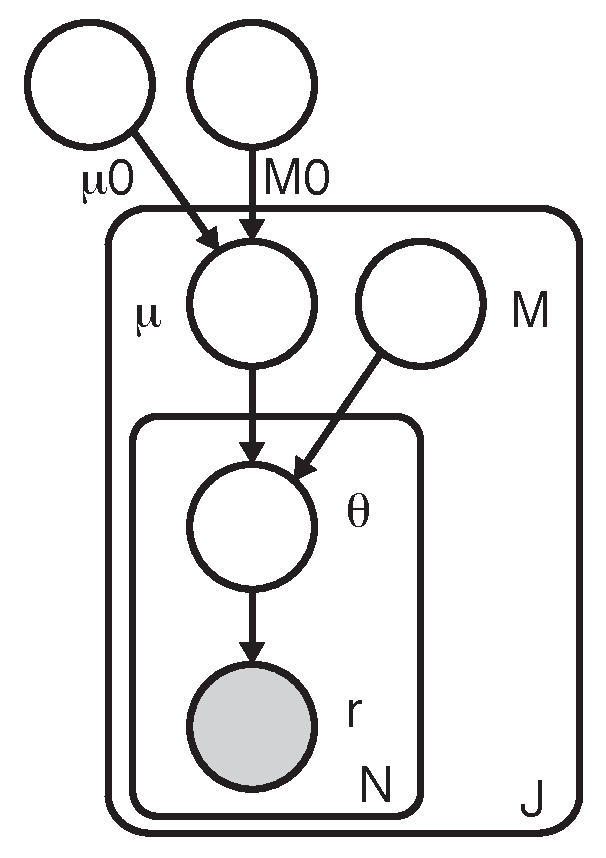
\includegraphics[width=40mm]{pdf_figs/RVD2_model.pdf}
\caption{RVD2 Graphical Model}
\label{fig:graphical_model}
\end{center}
\end{figure}


The joint distribution over the latent and observed variables for data at location $j$ in replicate $i$ given the parameters is

\begin{equation}\label{eqn:jointpdf}
p \left( r_{ji}, \theta_{ji}, \mu_j | n_{ji}; \mu_0, M_0, M_j \right) = p \left( r_{ji} | \theta_{ji}, n_{ji} \right) p\left( \theta_{ji} | \mu_j; M_j \right) p\left( \mu_j; \mu_0, M_0 \right),
\end{equation}

where
\begin{align}
p\left( \mu_j; \mu_0, M_0 \right)  &= \frac{ \Gamma(M_0) } { \Gamma(\mu_0 M_0) \Gamma(M_0 (1-\mu_0)) } \mu_j^{M_0\mu_0 -1} (1 - \mu_j)^{M_0 ( 1 - \mu_0) - 1}, \nonumber \\
p\left( \theta_{ji} | \mu_j; M_j \right) &= \frac{ \Gamma(M_j) } { \Gamma(\mu_j M_j) \Gamma(M_j (1-\mu_j)) } \theta_{ji}^{M_j\mu_j -1} (1 - \theta_{ji})^{M_j ( 1 - \mu_j) - 1}, \nonumber \\
p \left( r_{ji} | \theta_{ji}, n_{ji} \right) &= \frac{ \Gamma(n_{ji}+1) } { \Gamma(r_{ji}+1) \Gamma( n_{ji} - r_{ji} + 1 ) } \theta_{ji}^{r_{ji}} (1 - \theta_{ji})^{n_{ji} - r_{ji}}. \nonumber
\end{align}

Integrating over the latent variables $\theta_{ji}$ and $\mu_j$ yields the marginal distribution of the data,
\begin{equation}
p \left( r_{ji} | n_{ji} ; \mu_0, M_0, M_j \right) = \int_{\mu_j} \int_{\theta_{ji}}  p \left( r_{ji} | \theta_{ji}, n_{ji} \right) p\left( \theta_{ji} | \mu_j; M_j \right) p\left( \mu_j; \mu_0, M_0 \right) d\theta_{ji} d\mu_j.
\end{equation}

Finally, the log-likelihood of the data set is

\begin{equation}
\log p \left( r | n ; \mu_0, M_0, M \right) = \sum_{j=1}^J \sum_{i=1}^N \log \int_{\mu_j} \int_{\theta_{ji}}  p \left( r_{ji} | \theta_{ji}, n_{ji} \right) p\left( \theta_{ji} | \mu_j; M_j \right) p\left( \mu_j; \mu_0, M_0 \right) d\theta_{ji} d\mu_j.
\end{equation}



%%%%%%%%%%%%%%%%%%
% Variational approach
%%%%%%%%%%%%%%%%%%
\section{Variational theory}

\subsection{Factorization} 

We propose the following factorized variational distribution to approximate the true posterior over latent variables:
\begin{equation}
  q(\mu, \theta) = q(\mu)q(\theta) = \prod_{j=1}^J q(\mu_{j}) \prod_{i=1}^N q(\theta_{ji}).
  \label{eq:vardist}
\end{equation}


\subsection{Derivation of $ q(\mu) $ and $ q(\theta) $}

\subsubsection{Derivation of $ q(\theta) $}

\begin{equation}
\begin{split}
\log q_\theta^*(\theta) &= E_\mu\left[ \log p\left(r,\mu,\theta | n; \phi \right) \right] \\
&= E_\mu \left[ \log p\left(r | \theta, n \right)\right] + E_\mu \left[ \log p\left(\theta | \mu; M \right)\right] + E_\mu \left[ \log p\left(\mu ; \mu_0, M_0 \right)\right] \\
&= \sum_{j=1}^{J} \sum_{i=1}^{N} E_\mu  \left[ \log p \left( r_{ji} | \theta_{ji}, n_{ji} \right) \right] + \sum_{j=1}^{J} \sum_{i=1}^{N} E_\mu \left[ \log p\left(\theta_{ji} | \mu_j; M_j \right)\right] +con. \\
&= \sum_{j=1}^{J} \sum_{i=1}^{N}  E_\mu  \left[ \log \left( \frac{ \Gamma(n_{ji}+1) } { \Gamma(r_{ji}+1) \Gamma( n_{ji} - r_{ji} + 1 ) } \theta_{ji}^{r_{ji}} (1 - \theta_{ji})^{n_{ji} - r_{ji}} \right) \right] \\
&\quad + \sum_{j=1}^{J} \sum_{i=1}^{N}  E_\mu  \left[ \log \left( \frac{ \Gamma(M_j) } { \Gamma(\mu_j M_j) \Gamma(M_j (1-\mu_j)) } \theta_{ji}^{M_j\mu_j -1} (1 - \theta_{ji})^{M_j ( 1 - \mu_j) - 1} \right) \right] +con.\\
&=  \sum_{j=1}^{J} \sum_{i=1}^{N} E_\mu\left[ \log \left( \theta_{ji}^{r_{ji} + M_j\mu_j -1} (1 - \theta_{ji})^{n_{ji} - r_{ji} + M_j ( 1 - \mu_j) - 1} \right) \right] +con. \\
&=   \sum_{j=1}^{J} \sum_{i=1}^{N} \left[ \log \left( \theta_{ji}^{r_{ji} + M_j E_\mu\left[ \mu_j\right] -1} (1 - \theta_{ji})^{n_{ji} - r_{ji} + M_j ( 1 - E_\mu\left[ \mu_j\right]) - 1} \right) \right] +con. \\
\end{split}
\end{equation}

Exponentiating both sides, we can see that  $ q_\theta^*(\theta) $ is a product of beta distributions:
\begin{align}
\theta_{ji} \thicksim \text{Binomial}(\alpha_{ji}, \beta_{ji})
\end{align}
where,
\begin{align}
\alpha_{ji} &= r_{ji} + M_j E_\mu\left[ \mu_j\right] -1 \nonumber \\
\beta_{ji} &= n_{ji} - r_{ji} + M_j ( 1 - E_\mu\left[ \mu_j\right]) \nonumber
\end{align}


\subsubsection{Derivation of $ q(\mu) $}
\begin{equation}
\label{now}
\begin{split}
\log q_\mu^*(\mu) &= E_\theta\left[ \log p\left(r,\mu,\theta | n; \phi \right) \right] \\
&= E_\theta \left[ \log p\left(r | \theta, n \right)\right] + E_\theta \left[ \log p\left(\theta | \mu; M \right)\right] + E_\theta \left[ \log p\left(\mu ; \mu_0, M_0 \right)\right] \\
&= \sum_{j=1}^{J} \sum_{i=1}^{N} E_\theta \left[ \log p\left(\theta_{ji} | \mu_j; M_j \right)\right] + \sum_{j=1}^{J} E_\theta  \left[ \log p\left( \mu_j; \mu_0, M_0 \right) \right] + con.\\
&= \sum_{j=1}^{J} \sum_{i=1}^{N}  E_\theta  \left[ \log \left( \frac{ \Gamma(M_j) } { \Gamma(\mu_j M_j) \Gamma(M_j (1-\mu_j)) } \theta_{ji}^{M_j\mu_j -1} (1 - \theta_{ji})^{M_j ( 1 - \mu_j) - 1} \right) \right] \\
&\quad + \sum_{j=1}^{J} E_\theta  \left[ \log \left( \frac{ \Gamma(M_0) } { \Gamma(\mu_0 M_0) \Gamma(M_0 (1-\mu_0)) } \mu_j^{M_0\mu_0 -1} (1 - \mu_j)^{M_0 ( 1 - \mu_0) - 1} \right) \right] + con. \\
&= \sum_{j=1}^{J} \log \left( \frac{ \Gamma(M_j) } { \Gamma(\mu_j M_j) \Gamma(M_j (1-\mu_j)) }\right) \\
&\quad + \sum_{j=1}^{J} \sum_{i=1}^{N} \left\lbrace  \left( M_j\mu_j -1\right) E_\theta  \left[ \log \theta_{ji}\right] + \left( M_j ( 1 - \mu_j) - 1 \right)  E_\theta  \left[ \log \left( 1- \theta_{ji}\right) \right] \right\rbrace \\
&\quad + \sum_{j=1}^{J} \left\lbrace (M_0 \mu_0 - 1) \log \mu_j + (M_0 ( 1 - \mu_0) - 1) \log ( 1 - \mu_j)\right\rbrace  + con. \\
\end{split}
\end{equation}

It can be seen that the distribution function of $ q_\mu^*(\mu) $ is not any known distribution. We propose to approximate $ q_\mu^*(\mu) $ using Beta distribution.
\begin{align}
\mu_j \thicksim \text{Beta}(\delta_j, \gamma_j)
\end{align}
where,
\begin{align}
\delta_j &=  \nonumber \\
\gamma_j &=  \nonumber
\end{align}



\subsection{ELBO compute}

Using Jensen's inequality, the log-likelihood of the data is lower-bounded:

\begin{equation}
\begin{split}
\log p \left( r | \phi \right) &= \log \int_\mu \int_\theta p\left(r,\mu,\theta \right) d\theta d\mu \\ 
&= \log \int_\mu \int_\theta p\left(r,\mu,\theta \right)\frac{q\left(\mu,\theta \right) }{q\left(\mu,\theta \right) } d\theta d\mu \\ 
&\geq \int_\mu \int_\theta q\left(\mu,\theta \right) \log \frac{ p\left(r,\mu,\theta \right)}{q\left(\mu,\theta \right)} d\theta d\mu \\
&= E_q \left[ \log p\left(r,\mu,\theta \right)\right] - E_q \left[ \log q\left(\mu,\theta \right)\right] \\
&\triangleq \mathcal{L}(q, \phi) ,
\end{split}
\end{equation}

where $ \phi= \left( \mu_0, M_0, M \right) $

Actually, 

\begin{equation}
\begin{split}
\log p \left( r | \phi \right) &= \log \int_\mu \int_\theta p\left(r,\mu,\theta \right) d\theta d\mu \\ 
&= \log \int_\mu \int_\theta p\left(r,\mu,\theta \right)\frac{q\left(\mu,\theta \right) }{q\left(\mu,\theta \right) } d\theta d\mu \\ 
&= \int_\mu \int_\theta q\left(\mu,\theta \right) \log \frac{ p\left(r,\mu,\theta \right)}{q\left(\mu,\theta \right)} d\theta d\mu - \int_\mu \int_\theta q\left(\mu,\theta \right) \log \dfrac{p\left( \mu, \theta | r\right) }{q\left(\mu,\theta \right)} d\theta d\mu \\
&= \mathcal{L}(q, \phi) + KL\left(q(\mu,\theta ) || p( \mu, \theta | r) \right) ,
\end{split}
\end{equation}

Maximizing the ELBO is equivalent to minimizing the KL-divergence between the variational distribution and the true posterior.


Writing out ELBO $ \mathcal{L}(q, \phi) $, we have
\begin{equation}
\begin{split}
\label{L}
\mathcal{L}(q, \phi) &= E_q \left[ \log p\left(r,\mu,\theta | n; \phi \right)\right] - E_q \left[ \log q\left(\mu,\theta \right)\right] \\
&= E_q \left[ \log p\left(r | \theta, n \right)\right] + E_q \left[ \log p\left(\theta | \mu; M \right)\right] + E_q \left[ \log p\left(\mu ; \mu_0, M_0 \right)\right]- E_q \left[ \log q\left(\mu \right)\right]- E_q \left[ \log q\left(\theta \right)\right] \\
\end{split}
\end{equation}

\begin{equation}
\begin{split}
\label{r}
E_q \left[ \log p\left(r | \theta, n \right)\right] &= \sum_{j=1}^{J} \sum_{i=1}^{N} E_q  \left[ \log p \left( r_{ji} | \theta_{ji}, n_{ji} \right) \right] \\
&= \sum_{j=1}^{J} \sum_{i=1}^{N}  E_q  \left[ \log \left( \frac{ \Gamma(n_{ji}+1) } { \Gamma(r_{ji}+1) \Gamma( n_{ji} - r_{ji} + 1 ) } \theta_{ji}^{r_{ji}} (1 - \theta_{ji})^{n_{ji} - r_{ji}} \right) \right] \\
&= \sum_{j=1}^{J} \sum_{i=1}^{N}  E_q  \left[ r_{ji} \log \theta_{ji} + (n_{ji} - r_{ji}) \log (1 - \theta_{ji}) \right] + con. \\
&= \sum_{j=1}^{J} \sum_{i=1}^{N} \left\lbrace r_{ji} E_q \left[ \log \theta_{ji} \right] + (n_{ji} - r_{ji}) E_q  \left[  \log (1 - \theta_{ji}) \right] \right\rbrace + con. \\
\end{split}
\end{equation}

\begin{equation}
\begin{split}
\label{theta}
E_q \left[ \log p\left(\theta | \mu; M \right)\right] &= \sum_{j=1}^{J} \sum_{i=1}^{N} E_q \left[ \log p\left(\theta_{ji} | \mu_j; M_j \right)\right] \\
&= \sum_{j=1}^{J} \sum_{i=1}^{N}  E_q  \left[ \log \left( \frac{ \Gamma(M_j) } { \Gamma(\mu_j M_j) \Gamma(M_j (1-\mu_j)) } \theta_{ji}^{M_j\mu_j -1} (1 - \theta_{ji})^{M_j ( 1 - \mu_j) - 1} \right) \right] \\
%
&= \sum_{j=1}^{J} E_q  \left[ \log \left( \frac{ \Gamma(M_j) } { \Gamma(\mu_j M_j) \Gamma(M_j (1-\mu_j)) }\right) \right] + \sum_{j=1}^{J} \sum_{i=1}^{N}  E_q  \left[ \log \left( \theta_{ji}^{M_j\mu_j -1} (1 - \theta_{ji})^{M_j ( 1 - \mu_j) - 1} \right) \right] \\
%
&= \sum_{j=1}^{J} E_q  \left[ \log \left( \frac{ \Gamma(M_j) } { \Gamma(\mu_j M_j) \Gamma(M_j (1-\mu_j)) }\right) \right]  \\ 
&\quad + \sum_{j=1}^{J} \sum_{i=1}^{N} \left\lbrace E_q \left[ \left( M_j\mu_j -1 \right) \log \theta_{ji} \right] + E_q \left[ \left( M_j ( 1 - \mu_j) - 1 \right) \log \left( 1 - \theta_{ji} \right) \right]\right\rbrace \\
%
&= \sum_{j=1}^{J} E_q  \left[ \log \left( \frac{ \Gamma(M_j) } { \Gamma(\mu_j M_j) \Gamma(M_j (1-\mu_j)) }\right) \right] \\ 
&\quad + \sum_{j=1}^{J} \sum_{i=1}^{N} \left\lbrace M_j E_q \left[ \mu_j \right] E_q \left[ \log \theta_{ji} \right] - E_q  \left[ \log \theta_{ji} \right] + \left( M_j - 1 - M_j E_q\left[ \mu_j \right]  \right) E_q\left[ \log \left( 1 - \theta_{ji}\right) \right] \right\rbrace \\
%
%&= \sum_{j=1}^{J}  \left\lbrace \log \Gamma(M_j) - E_q  \left[ \log \Gamma(\mu_j M_j) \right] + E_q  \left[ \log \Gamma(M_j (1-\mu_j)) \right] \right\rbrace \\ 
%&\quad + \sum_{j=1}^{J} \sum_{i=1}^{N} \left\lbrace E_q \left[ \left( M_j\mu_j -1 \right) \log \theta_{ji} \right] + E_q \left[ \left( M_j ( 1 - \mu_j) - 1 \right) \log \left( 1 - \theta_{ji} \right) \right]\right\rbrace \\
%
%&= \sum_{j=1}^{J}  \left\lbrace E_q  \left[ \log \Gamma(M_j) \right] - E_q  \left[ \log \Gamma(\mu_j M_j) \right] + E_q  \left[ \log \Gamma(M_j (1-\mu_j)) \right] \right\rbrace \\ 
%&\quad + \sum_{j=1}^{J} \sum_{i=1}^{N} \left\lbrace M_j E_q \left[ \mu_j \right] E_q \left[ \log \theta_{ji} \right] - E_q  \left[ \log \theta_{ji} \right] + \left( M_j - 1 - M_j E_q\left[ \mu_j \right]  \right) E_q\left[ \log \left( 1 - \theta_{ji}\right) \right] \right\rbrace \\
\end{split}
\end{equation}

\begin{equation}
\begin{split}
\label{mu}
E_q \left[ \log p\left(\mu ; \mu_0, M_0 \right)\right] &= \sum_{j=1}^{J} E_q  \left[ \log p\left( \mu_j; \mu_0, M_0 \right) \right] \\
&= \sum_{j=1}^{J} E_q  \left[ \log \left( \frac{ \Gamma(M_0) } { \Gamma(\mu_0 M_0) \Gamma(M_0 (1-\mu_0)) } \mu_j^{M_0\mu_0 -1} (1 - \mu_j)^{M_0 ( 1 - \mu_0) - 1} \right) \right] \\
&= \log \frac{ \Gamma(M_0) } { \Gamma(\mu_0 M_0) \Gamma(M_0 (1-\mu_0))} \\
&\quad + \sum_{j=1}^{J} \left\lbrace (M_0\mu_0 -1)E_q  \left[ \log \mu_j \right] + (M_0 ( 1 - \mu_0) - 1) E_q  \left[ \log (1 - \mu_j)\right]\right\rbrace  \\
%
%&= \left\lbrace \log \Gamma(M_0) - \log \Gamma(\mu_0 M_0) - \log \Gamma(M_0 (1-\mu_0))\right\rbrace \\
%&\quad + \sum_{j=1}^{J} \left\lbrace (M_0\mu_0 -1)E_q  \left[ \log \mu_j \right] + (M_0 ( 1 - \mu_0) - 1) E_q  \left[ \log (1 - \mu_j)\right]\right\rbrace  \\
%
\end{split}
\end{equation}

Therefore, in order to compute ELBO, we need to compute the following expectations with respect to variational distribution: $ E_q \left[ \log \theta_{ji} \right] $, $ E_q\left[ \log \left( 1 - \theta_{ji}\right) \right] $ , $ E_q  \left[ \log \mu_j \right] $ , $ E_q  \left[ \log (1 - \mu_j)\right] $, $ E_q \left[ \mu_j \right] $ , $ E_q  \left[ \log \left( \frac{ \Gamma(M_j) } { \Gamma(\mu_j M_j) \Gamma(M_j (1-\mu_j)) }\right) \right] $.

From 
\begin{align}
\theta_{ji} &\thicksim \text{Binomial}(\alpha_{ji}, \beta_{ji}) \nonumber \\
\mu_j &\thicksim \text{Beta}(\delta_j, \gamma_j) \nonumber
\end{align}

We know
\begin{align}
E_q \left[ \log \theta_{ji} \right] &= \psi(\alpha_{ji}) - \psi(\beta_{ji}) \nonumber \\
E_q\left[ \log \left( 1 - \theta_{ji}\right) \right]&= \nonumber \\
E_q \left[ \mu_j \right] &= \frac{\delta_j}{\delta_j + \gamma_j} \nonumber \\
E_q  \left[ \log \mu_j \right] &= \psi(\delta_j) - \psi(\gamma_j) \nonumber \\
E_q  \left[ \log (1 - \mu_j)\right] &= \nonumber \\
E_q  \left[ \log \left( \frac{ \Gamma(M_j) } { \Gamma(\mu_j M_j) \Gamma(M_j (1-\mu_j)) }\right) \right]&= \nonumber 
\end{align}

\subsubsection{LIB function Approximation} \

There are two conditions that we are satisfied:
\begin{enumerate}[noitemsep]
	\item the trigamma function $ \psi ' (.)  $ is a positive monotonously decreasing function;
	\item For each location $j$:
\end{enumerate}


%\bibliographystyle{apalike}
%\bibliography{bioinfo}
\end{document}
